\documentclass[journal]{IEEEtran}

\usepackage[pdftex]{graphicx}
\graphicspath{{img/}}
\usepackage{cite}
\usepackage{amsmath}
\usepackage{mathtools}
\usepackage{booktabs,siunitx}
\usepackage{threeparttable}
%\usepackage{subcaption}
\usepackage{multirow}
\usepackage[caption=false,font=footnotesize,labelfont=sf,textfont=sf]{subfig}

% TODO: remove
	\usepackage{xcolor}
	\newcommand\TODO[1]{\textcolor{red}{TODO: #1}}

\begin{document}
\title{Title of the Paper}


\author{Michael~Mueller,
        Jan~Riedo,
        Michael~Rebsamen% <-this % stops a space
\thanks{Biomedical Engineering, University of Bern}% <-this % stops a space
\thanks{Authors e-Mail: michael.mueller@students.unibe.ch, jan.riedo@students.unibe.ch, michael.rebsamen@students.unibe.ch}}% <-this % stops a space
\markboth{Biomedical Engineering, Medical Image Analysis Lab, \today}%
{Title of the Paper}
\maketitle

\begin{abstract}
Bla
\end{abstract}

\section{Introduction}
\TODO{MR: Understand clinical problem, technical requirements (e.g. allow randomisation), Anatomy}

kNN is a popular classification method for MR data and has successfully been applied in MR brain segmentation\cite{Anbeek2004,Cocosco2003,Warfield2000}


\section{Methods}

\subsection{Dataset}
All experiments were conducted on a subset of 100 unrelated subjects from a dataset provided by the \textit{Human Connectome Project} \cite{van2013wu}. From each individual, a total of eight 3-tesla head MRI are available: T1 and T2-weighted image volumes not skull-stripped (but defaced for anonymization) and skull-stripped with a bias field correction, and both modalities once in native T1 space and once in MNI-atlas space \cite{mazziotta2001probabilistic}.

Ground-truth labels are automatically generated using \textit{FreeSurf}, assigning each voxel either to background, white matter, grey matter, or ventricles. The dataset was split in a training set with 70 images and a test set with 30 images.
\subsection{Pipeline}
\TODO{Describe whole pipeline (registration, pre-processing, feature extraction, ML classification, post-processing, evaluation}

\subsection{Training}
\TODO{Describe training of machine learning algorithms}

\subsection{Performance Evaluation}
\TODO{Describe metric (dice score)}

\subsection{Infrastructure}
\TODO{Describe UBELIX, libraries}


\section{Results}

\TODO{JR: DF hyperparameter optimization, 3DPlot}
The decision forest algorithm was enhanced with normalized features, a higher number of ventricle voxels in the training set and the optimization of the hyperparameters (see Fig.~\ref{f.df_white}). With this settings, the max dice coefficient was lifted from 0.703 to 0.754. This result was achieved with 80 trees and 3000 max nodes.

\begin{figure}[h!]\label{f.df_white}
	\centering
	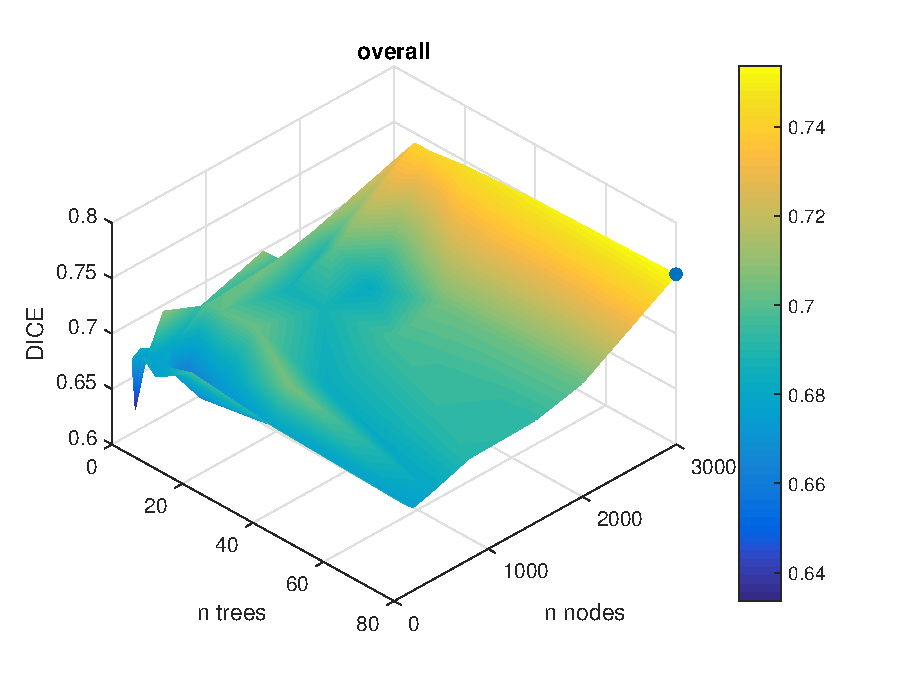
\includegraphics[width=0.48\textwidth]{images/DF_crossval}
	\caption{Mean dice of white/grey matter and ventricles based on the hyperparameters number of trees and maximum nodes.}
\end{figure}

\TODO{JR: kNN optimization}


\TODO{JR: overall result table}\\


\begin{table}[h!]
	\begin{center}
		\label{tab.dice}
		\caption{Best dice score of each algorithm after optimization and score of ensemble.}
		\begin{tabular}{c|ccc|c}
			algorithm &             \multicolumn{4}{c}{dice}              \\ \cline{2-5}
			          & white matter & grey matter & ventricles & overall \\
			   DF     &              &             &            &  \\
			   SVM    &              &             &            &  \\
			   kNN    &              &             &            &  \\
			   SGD    &              &             &            &  \\
			   GMM    &              &             &            &  \\
			ensemble  &              &             &            &
		\end{tabular}
	\end{center}
DF: Decision Forest, SVM: Support Vector Machine, kNN: k Nearest Neighbor, SGD: Stochastic Gradient Descent, GMM: Gaussian Mixture Model.
\end{table} 

\begin{table*}[t]
\renewcommand{\arraystretch}{1.2}
\newcommand\mulrow[2]{\multirow{#1}{*}{\shortstack[c]{#2}}}
\caption{Performance Comparison of ML Algorithms}
\label{tab:perf_compare}
\centering
\begin{threeparttable}
\begin{tabular*}{0.9\textwidth}{@{\extracolsep{\fill}}c*{6}{S[table-number-alignment=center,table-figures-decimal=2,table-auto-round]}@{}}
\toprule
Features & {Size Dataset} & {\shortstack[c]{DF}} & {\shortstack[c]{GMM}} & {\shortstack[c]{kNN}} & {\shortstack[c]{SGD}} & {\shortstack[c]{SVM}}\\
\midrule
\mulrow{3}{All\\(f1-f7)}
	& 3		&	{-}		& {-}	& {-}	& {-}	& {-}\\
	& 12		&	{0.84/0.80/0.52}		& {0.00/0.78/0.00}	& {0.81/0.78/0.33}	& {0.82/0.79/0.00}	& {0.84/0.80/0.46}\\
	& 70		&	{-}		& {-}	& {-}	& {-}	& {-}\\
\midrule
\mulrow{3}{Coordinates only\\(f1-f3)}
	& 3		&	{-}		& {-}	& {-}	& {-}	& {-}\\
	& 12		&	{-}		& {-}	& {-}	& {-}	& {-}\\
	& 70		&	{-}		& {-}	& {-}	& {-}	& {-}\\
\midrule
\mulrow{3}{All non-coordinates \\(f4-f7)}
	& 3		&	{-}		& {-}	& {-}	& {-}	& {-}\\
	& 12		&	{-}		& {-}	& {-}	& {-}	& {-}\\
	& 70		&	{-}		& {-}	& {-}	& {-}	& {-}\\
\bottomrule
\end{tabular*}
\begin{tablenotes}
\item Overview of achieved accuracy for the different algorithms. Mean dice scores for white matter/grey matter/ventricles.
\item f1-f3: Coordinate features, f4: T1 intensity, f5: T1 gradient, f6: T2 intensity, f7: T2 gradient.
\end{tablenotes}
\end{threeparttable}
\end{table*}

\section{Discussion}
\TODO{challenge with quality of ground truth}

\TODO{feature importance}


\section{Conclusion}

\section*{Acknowledgment}

\bibliographystyle{IEEEtran}
\bibliography{references}

\end{document}